% -------------------- Packages --------------------

\documentclass[a4paper, 12pt]{ctexart}

\RequirePackage{enumerate}
\RequirePackage{fontspec} % fonts.
\RequirePackage[dvipsnames]{xcolor} % color declarations.

\RequirePackage{amsmath}
\RequirePackage{amssymb}
\RequirePackage{commath} % abs, norm

\RequirePackage[amsmath]{ntheorem} % 定理格式.

\theoremstyle{plain}
\newtheorem{problem}{问题}

\theoremstyle{nonumberplain}
\newtheorem{proof}{证明}
\newtheorem{solution}{解}
\newtheorem{hint}{提示}
\newtheorem{analysis}{分析}
\newtheorem{supplement}{拓展}
\newtheorem{example}{例}
\newtheorem{category}{考点}

\usepackage{xparse}
\usepackage{xtemplate}
\usepackage{tasks}

\settasks{label=(\Alph*), label-width=1.6em}

\RequirePackage{graphicx}

% -------------------- Settings --------------------

% -------------------- New commands --------------------

\newcommand{\ans}[1]{\textcolor{Aquamarine}{#1}}
\newcommand{\doubt}[1]{\textcolor{Red}{#1}}

\newcommand*{\diff}{\mathop{}\!\mathrm{d}}
\newcommand*{\vect}[1]{\mathbf{#1}}
\newcommand{\me}{\mathrm{e}}
\newcommand{\BR}{\mathbb{R}}
\newcommand{\BN}{\mathbb{N}}

\newcommand{\lr}[3]{\left#1#3\right#2}
\newcommand{\lmr}[5]{\left#1#4\middle#2#5\right#3}

\newcommand{\efootnote}[1]{\footnote{菜鸡注: #1}}

% 我觉得主要用到的就是 定理环境 \ans命令 以及tasks包

% -------------------- Document --------------------

\begin{document}

\section{胡诗敏}

\begin{problem}
    函数$f(x)$在$[x_0, +\infty)$上具有二阶导数, 并且$f''(x)<0$, 对于任意$x>x_0$, 由拉格朗日中值定理, 存在$\xi\in (x_0, x)$, 使得$f(x)-f(x_0)=f'(\xi)(x-x_0)$. 证明$\xi$定义了$(x_0, +\infty)$上的一个单调增加函数.
\end{problem}
\begin{category}
    拉格朗日中值定理; 函数的定义; 导数.
\end{category}
\begin{analysis}
    这道题的要求有两个关键点:
    \begin{itemize}
        \item 证明$\xi$关于$x$是一个函数: 根据函数的定义, 一个自变量对应唯一的因变量, 所以由$f'(x)$递减, $\xi=\xi(x)$可以唯一确定(函数).\efootnote{我个人认为这里分析写的不对, 我们不需要证明对于每一个$x$, 只存在一个中值点$\xi$. 题目中已经写得足够详细了, 所以我不打算对函数$\overline{\xi}$的构造再做解释. 各位可以回顾一下一道类似的构造数列的习题, "若$x_n$是无界数列, 证明: 可以找到单调递增的子数列$\{x_{n_k}\}$使得$x_{n_k} > k$." 要知道数列实际上就是正整数集到实数集的映射, 而当时通过$x_{n_k}$找$x_{n_{k+1}}$的时候也没有要求唯一性. 希望大家能好好理解一下函数的概念, 理解一下一阶逻辑(全称量词和存在量词), 能学学选择公理就最好了.}
        \item 证明函数单增: 因为$\lmr./.{\lr(){f(x)-f(x_0)}}{\lr(){x-x_0}}$递减, 可得$\xi(x)$递增.
    \end{itemize}
\end{analysis}
\begin{proof}
    任取$x>0$, 存在$\xi\in(x_0, x)$, 使得$f(x)-f(x_0)=f'(\xi)(x-x_0)$. 又因为$f'(x)$是单调递减函数, 所以$\xi$唯一, 有$\xi=\xi(x)$, $x\in(x_0, +\infty)$. 令
    \begin{equation}
        F(x) = \frac{f(x)-f(x_0)}{x-x_0},
    \end{equation}
    则
    \begin{equation}
        F'(x) = \frac{f'(x)(x-x_0)- (f(x)-f(x_0))}{(x-x_0)^2}.
    \end{equation}
    令
    \begin{equation}
        g(x) = f'(x)(x-x_0)-(f(x)-f(x_0)),
    \end{equation}
    则
    \begin{equation}
        g'(x) = f''(x)(x-x_0)+f'(x)-f'(x) = f''(x)(x-x_0).
    \end{equation}
    当$x>0$时, 有$f''(x)<0$, $g'(x)<0$, $g(x)$单减, $g(x_0)=0$, 所以$g(x)<0$, $F'(x)<0$, $F(x)$单减, $f'(x) = F(x)$. 因为$F(x)$递减, $f'(x)$递减, 所以$\xi=\xi(x)$递减.\efootnote{原文就这么乱.}
\end{proof}

\begin{problem}
    试说明闭区间上连续函数的像集是闭区间.
\end{problem}
\begin{category}
    连续函数的性质.
\end{category}
\begin{analysis}
    做这道题首先得理解像集是闭区间的含义, 然后联想连续函数的性质, 发现根据最值原理和介值定理可以做出.\efootnote{连续函数把闭区间映到闭区间其实是两条性质的反映, 第一条是连续函数把连通集映到连通集, 也就是大家熟悉的介值定理; 第二条是连续函数把闭集映到闭集, 也就是说连续函数把收敛序列映到收敛序列. 可能是一种不一样的理解方式吧.}
\end{analysis}
\begin{proof}
    设有连续函数$f(x)$, $x\in [a, b]$, 设其像集为$A$, 根据连续函数的最值定理, $f(x)$在$[a, b]$上可以取到最大值$M$和最小值$m$, 有$A\subseteq[m, M]$. 不妨设$f(x_1)=M$, $f(x_2)=m$, $x_1, x_2\in[a, b]$, $x_1<x_2$.\efootnote{不妨想一想这里为什么可以不妨设.}根据连续函数的介值定理, 任取$\eta\in[m, M]$, 存在$x\in [x_1, x_2]$, 使得$f(x)=\eta$, 则$[m, M]\subseteq A$.\efootnote{如果想要证明两个集合$E$和$F$相等, 基本的想法就是证明$E$包含$F$以及$F$包含$E$, 希望大家能记住.} 综上, 该函数的像集是闭区间$[m, M]$.
\end{proof}

\begin{problem}
    $f(x)$具有二阶导数, 如果极限
    \begin{equation}
        \lim_{x\to 0}\frac{1+f(x)+xf(2x)}{x^2}=-1,
    \end{equation}
    求$f(0)$, $f'(0)$, $f''(0)$.
\end{problem}
\begin{category}
    泰勒公式; 极限; 洛必达法则的使用条件(如果不注意这一点, 虽然有可能得出正确的答案, 但解题过程却有可能是错误的)
\end{category}
\begin{analysis}
    这道题比较简单的方法是, 直接写出$f(x)$在0点处的带有佩亚诺余项的泰勒公式, 然后依次求出$f(0)$, $f'(0)$, $f''(0)$. 下面给出另外一种方法, 可能不是很简洁, 但希望大家能通过下面这种做法加深对洛必达法则使用条件的印象.
\end{analysis}
\begin{solution}
    根据极限的四则运算法则得
    \begin{equation}
        \lim_{x\to 0}[1+f(x)+xf(2x)]=0.
    \end{equation}
    由于$f(x)$具有二阶导数, 故$f(x)$连续, 有
    \begin{equation}
        0 = \lim_{x\to 0}[1+f(x)+xf(2x)] = 1+f(0),
    \end{equation}
    故$f(0)=-1$. 根据极限的四则运算法则得
    \begin{equation}
        \lim_{x\to 0}\frac{1+f(x)+xf(2x)}{x}=0.
    \end{equation}
    且注意到$f'(x)$连续, 可得
    \begin{equation}
        0 = \lim_{x\to 0}\frac{1+f(x)+xf(2x)}{x}=\lim_{x\to 0}\frac{f'(x)+f(2x)+2xf'(2x)}{1} = f'(0) + f(0).
    \end{equation}
    故$f'(0)=1$. 则当$x\to 0$时, 有
    \begin{equation}
        f(x) = f(0) + f'(0)x + \frac{1}{2}f''(0)x^2 + o(x^2) = -1 + x + \frac{1}{2}f''(0)x^2 + o(x^2).
    \end{equation}
    故
    \begin{equation}
        -1 = \lim_{x\to 0}\frac{1+f(x)+xf(2x)}{x^2} = \lim_{x\to 0}\frac{f''(0)x^2+4x^2+o(x^2)}{2x^2}= \frac{1}{2}f''(0)+2.
    \end{equation}
    故$f''(0)=-6$(注意理解为什么求二阶导数时不能用和求$f(0)$, $f'(0)$类似的方法).
\end{solution}

\begin{problem}
    设$f(x) = x(x^2-1)(x^2-2)(x^2-3)+4$, 则$f(x)$在区间$(-2, 2)$内有几个极值点.
    \begin{tasks}(4)
        \task 3.
        \task 4.
        \task[\ans{(C)}] \ans{5}.
        \task 6.
    \end{tasks}
\end{problem}
\begin{analysis}
    这道题研究函数的极值点, 我们可以注意到这个函数的导数并不是很方便求, 但是通过绘制图像的方法, 可以较为快速的解出这道题目. 由于常数项与函数极值点无关, 可以根据零点快速准确地绘制$g(x)=x(x^2-1)(x^2-2)(x^3-3)$的图像, 然后判断出极值点的个数.\efootnote{TL;DR: 我觉得这种做法只在$g$没有复根也没有实重根的时候才适用, 可能是我太菜了. 正文: 我们来整理一下这种做法为什么正确, 用到了哪些定理. 设多项式$p$的次数为$n$, 且$p$有$n$个不同的实零点. 对于每两个相邻零点使用中值定理, 可以找到$p'$的$n-1$个两两不同的根. 而$p'$是$n-1$次多项式, 根据代数学基本定理, $p'$有且仅有$n-1$个复根(重根按重数记), 所以我们已经找到了$p'$的所有零点. 同样利用中值定理和代数学基本定理可以证明$p''$的零点集与$p'$的零点集不交, 所以$p'$的每个零点都是$p$的极值点, 因此我们可以画出合适的示意图.}
\end{analysis}
\begin{figure}[htb]
    \centering
    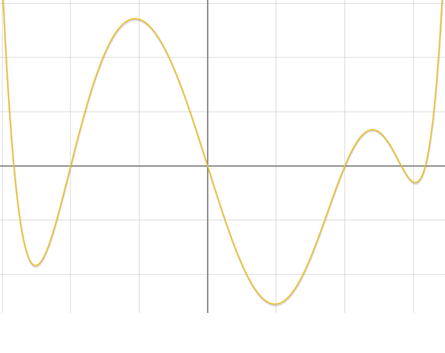
\includegraphics[width=7cm]{wsm.png}
    \caption{$g(x)=x(x^2-1)(x^2-2)(x^3-3)$示意图.}
\end{figure}

\section{陶一豪}

\begin{problem}
    若函数$f(x)$在$x=1$点可导, 且$f'(1)=-2$, 则极限
    \begin{equation}
        \lim_{x\to 0}\frac{f(\cos(x))-f(\cos(2x))}{x^2}=\ans{-3}.
    \end{equation}
\end{problem}
\begin{analysis}
    通过$\cos(x)-\cos(2x)=-(2\cos^2(x)-\cos(x)-1)$换出$f'(1)$, 再利用等价无穷小.
\end{analysis}

\begin{problem}
    单侧极限$A=f(x_0^+)$与单侧导数$B=f_+'(x_0)$的概念为
    \begin{tasks}(1)
        \task $A = \lim_{x\to x_0^+}f(x), B = \lim_{x\to x_0^+}f'(x)$
        \task $A = \lim_{\lr\vert\vert{\Delta x}\to 0}f(x_0+\Delta x), B = \lim_{\Delta x\to 0^+}\frac{f(x_0 + \Delta x) - f(x_0)}{\Delta x}$
        \task $A = \lim_{\lr\vert\vert{\Delta x \to 0}f(x_0 + \Delta x)}, B = \lim_{\Delta x \to 0}\frac{f(x_0 + \lr\vert\vert{\Delta x})-f(x_0)}{\Delta x}$
        \task[\ans{(D)}] \ans{$A = \lim_{\Delta x\to 0}f(x_0 + \lr\vert\vert{\Delta x}), B = \lim_{\Delta x \to 0}\frac{f(x_0 + \lr\vert\vert{\Delta x})- f(x_0)}{\lr\vert\vert{\Delta x}}$}
    \end{tasks}
\end{problem}
\begin{analysis}
    注意到$\lr\vert\vert{\Delta x}$上下均带绝对值的一定是在$x_0$右侧的某个域内, 符合定义.
\end{analysis}

\begin{problem}
    求常数$a$, 使得
    \begin{equation}
        f(x) =
        \begin{cases}
            \log(x+2),&x>0\\
            a^{x+b},&x\leq 0
        \end{cases}
    \end{equation}
    在$x=0$点可导.
\end{problem}
\begin{analysis}
    此题为将连续与导数的定义结合的题型, 一般是先根据可导必连续来判断出其中的一个值, 再根据左右导数相等来得出另一个值.
\end{analysis}
\begin{solution}
    因为$f(0^+)=\log(2)=f(0^-)=a^b$, $f_+'(0)=1/2=f_-'(0)=a^b\log(a)$, 因此$a = \exp(1/(2\log(2)))$
\end{solution}

\begin{problem}
    设函数$f(x)$在$x=0$的某邻域内具有连续导数, 且$f(0)\neq 0$, $f'(0)\neq 0$, 若$af(x) + bf(2x)-f(0)$在$x\to 0$时是比$x$高阶的无穷小, 试求常数$a, b$.
\end{problem}
\begin{solution}
    由$a+b-1=0, a+2b=0$知$a=2, b=-1$.
\end{solution}

\begin{problem}
    求由方程$x^3+y^3+(x+1)\cos(\pi y)+9=0$确定的隐函数的导数$y'$及$y'(-1)$.
\end{problem}
\begin{analysis}
    隐函数的求导往往是对一个方程进行左右两端同时求导, 求出来的$y'$可通过$x, y$对应的值来解出. 同理, 若求某一点的$y''$只需再次左右两端求导并代入相关的值.
\end{analysis}
\begin{solution}
    \begin{equation}
        y'= \frac{3x^2+\cos(\pi y)}{\pi(x+1)\sin(\pi y)-3y^2},\quad y(-1)=-\frac{1}{3}.
    \end{equation}
\end{solution}

\begin{problem}
    参数方程
    \begin{equation}
        \lr\{.{
            \begin{aligned}
                x &= 1+t^2\\
                y &= \cos(t)
            \end{aligned}
        }
    \end{equation}
    确定的函数的二阶导数
    \begin{equation}
        \frac{\diff^2y}{\diff x^2} = \ans{\frac{\sin(t)-t(\cos(t))}{4t^2}}.
    \end{equation}
\end{problem}
\begin{analysis}
    此题是参数方程的求导, 属于高频考察, 但只要不丢掉二阶导时的$x$, 再次求导并不难.
\end{analysis}

\begin{problem}
    $y = (x^4 + 1)\arctan(x^2)$, 则导数$y'= \ans{4x^3\arctan{x^2}+2x}$.
\end{problem}
\begin{analysis}
    此题是复合函数的求导, 只要谨记$f(g(x))$求导后不要忘了乘上$g'(x)$即可, 注意计算.
\end{analysis}

\begin{problem}
    函数
    \begin{equation}
        f(x) = \me^{2x^2 + 1}+ \sin(x)+ \frac{x\log(1+\arctan^6(x))}{\sqrt{2+x^2}}
    \end{equation}
    在$x=0$点的微分为
    \begin{tasks}(4)
        \task[\ans{(A)}] \ans{$\diff f(0) = \diff x$}
        \task $\diff f(0) = 2\diff x$
        \task $\diff f(0) = 3\diff x$
        \task $\diff f(0) = (\me + 1)\diff x$
    \end{tasks}
\end{problem}
\begin{analysis}
    耐心求导, 考验计算能力, 当然也可通过事先观察来判断出第一项与第三项求导后必定有$x$.
\end{analysis}

\begin{problem}
    设函数$f(x) = x^2\vert x\vert$, 使$f^{(n)}(0)$存在的最高阶数$n$的值为$\ans{2}$.
\end{problem}
\begin{analysis}
    想到在$0$处左右导数的求法
    \begin{equation}
        \lim_{x\to 0^+}\frac{f(x)- f(0)}{x} = \lim_{x\to 0^-}\frac{f(x)-f(0)}{x},
    \end{equation}
    在两端分析, 二阶导后由$f'''(0^+)=3$, $f'''(0^-)=-3$, 推出三阶导不存在, 那之后的导数也不存在.
\end{analysis}

\section{王硕}

\begin{problem}
    设$f(x)=\lr\vert\vert{x(x-1)^2(x-3)^3}$, 则$f(x)$的不可导点个数是
    \begin{tasks}(4)
        \task[\ans{(A)}] 1个
        \task 2个
        \task 3个
        \task 4个
    \end{tasks}
\end{problem}
\begin{category}
    函数可导的条件
\end{category}
\begin{analysis}
    同学们容易想当然地, 把绝对值里面的原来的函数的零点直接当做新函数的不可导点, 但是忽视了两种情况:
    \begin{enumerate}
        \item 在该零点(如x=1), 原函数的图像未穿过x轴.
        \item 在该零点(如x=3), 原函数的图像虽穿过x轴, 但在该点的导数值为0.
    \end{enumerate}
    加绝对值的意义就在于, 使原来函数的非极值的零点两侧的导数值由相等变为相反数, 要注意不能忽视0的相反数还是0, 所以以上的情况2依然可导.
\end{analysis}

\begin{problem}
    函数
    \begin{equation}
        y = \frac{2x-1}{x^2+3x-4}
    \end{equation}
    的$n$阶导数
    \begin{equation}
        \ans{y^{(n)} = \frac{(-1)^nn!}{5}\lr(){\frac{1}{(x-1)^{n+1}}+\frac{9}{(x+4)^{n+1}}}}.
    \end{equation}
\end{problem}
\begin{analysis}
    不经处理, 直接进行求导, 费时且做不出来. 应该先分解成$1/(kx+b)$的和的形式, 再利用公式求解.
\end{analysis}

\begin{problem}
    设$y=y(x)$是由方程
    \begin{equation}
        x = \int_1^{y-x}\sin^2(\frac{\pi t}{4})\diff t
    \end{equation}
    确定的隐函数, 则$y'(0)=\ans{3}$.
\end{problem}
\begin{category}
    隐函数求导, 变上限函数求导.
\end{category}
\begin{analysis}
    题目比较基础但是为必考点之一, 希望同学们通过一点练习来巩固这一知识点.
\end{analysis}

\end{document}
